\section{Results}
\label{sec:results}
In this section we describe the results obtained from our simulations.  The 
section is divided into two parts. In the first part we present some general 
results of our simulations, reviewing the general behaviour of our 
simulations. In the second part we present the results of our attempts to 
replicate the phenomena outlined in section~\ref{sec:article-results}. A 
discussion of these results is presented in section~\ref{sec:discussion}.

\subsection{The basics}
In this section we describe some general results of our simulations and the 
behaviour of our model. First we present the scenarios that we have simulated, 
and the parameters used in the simulations. We then move on to comment on the 
general behaviour of the pedestrians in our simulations and within which 
limits the simulations give reasonable results.

\subsubsection{Scenarios}
As outlined in section~\ref{sec:scenario-presentation}, we will simulate two 
different main scenarios, a square room and a corridor, with some variations 
of the latter. Counting these variations, we simulate four different 
scenarios: A rectangle shaped room with a door in the middle of one of the 
walls, and a normal corridor, a corridor with a bottleneck in the middle and a 
corridor with a sudden open space. In the corridors we do simulations of both 
uni-- and birectional flow. Images of each of these scenarios are presented in 
figure \ref{fig:fourcases}.

\begin{figure}[h]
    \centering
    \begin{minipage}{0.45\textwidth}
        \centering
        \subfloat[Square room.]{
        \resizebox{0.7\textwidth}{!}{\begin{tikzpicture}

\end{tikzpicture}
}
        \label{subfig:image-square-room}
        } 
        \\
        \subfloat[Corridor.]{
        \resizebox{\textwidth}{!}{\begin{tikzpicture}
\draw[color=blue] (11.86,0.21) circle (0.21);
\draw[color=blue] (12.23,-1.26) circle (0.19);
\draw[color=blue] (11.20,0.43) circle (0.21);
\draw[color=blue] (11.84,1.02) circle (0.20);
\draw[color=blue] (12.21,-0.58) circle (0.20);
\draw[color=blue] (10.65,0.54) circle (0.19);
\draw[color=blue] (11.47,-0.42) circle (0.20);
\draw[color=blue] (10.31,-0.21) circle (0.20);
\draw[color=blue] (10.09,0.52) circle (0.20);
\draw[color=blue] (9.67,-0.59) circle (0.21);
\draw[color=blue] (10.79,-0.65) circle (0.19);
\draw[color=blue] (8.99,-0.61) circle (0.17);
\draw[color=blue] (8.40,0.19) circle (0.20);
\draw[color=blue] (8.02,-0.08) circle (0.19);
\draw[color=blue] (9.02,-0.04) circle (0.18);
\draw[color=blue] (9.53,0.55) circle (0.19);
\draw[color=blue] (9.70,-0.02) circle (0.21);
\draw[color=blue] (8.54,-0.52) circle (0.20);
\draw[color=blue] (7.38,-0.12) circle (0.20);
\draw[color=blue] (7.99,-0.62) circle (0.20);
\draw[color=blue] (9.05,0.58) circle (0.19);
\draw[color=blue] (7.12,-0.63) circle (0.21);
\draw[color=blue] (6.73,-0.23) circle (0.20);
\draw[color=blue] (6.29,-0.68) circle (0.21);
\draw[color=blue] (6.99,0.51) circle (0.20);
\draw[color=blue] (5.63,-0.56) circle (0.20);
\draw[color=blue] (6.39,0.67) circle (0.21);
\draw[color=blue] (5.90,0.69) circle (0.20);
\draw[color=blue] (5.26,-0.79) circle (0.19);
\draw[color=blue] (6.07,-0.20) circle (0.21);
\draw[color=blue] (5.24,0.63) circle (0.20);
\draw[color=blue] (6.51,0.18) circle (0.19);
\draw[color=blue] (5.72,0.30) circle (0.21);
\draw[color=blue] (8.44,0.68) circle (0.19);
\draw[color=blue] (2.95,-0.67) circle (0.19);
\draw[color=blue] (4.81,-0.04) circle (0.23);
\draw[color=blue] (4.80,0.54) circle (0.19);
\draw[color=blue] (4.50,-0.67) circle (0.20);
\draw[color=blue] (7.76,0.48) circle (0.19);
\draw[color=blue] (3.48,0.17) circle (0.19);
\draw[color=blue] (5.48,-0.06) circle (0.21);
\draw[color=blue] (2.24,-0.57) circle (0.19);
\draw[color=blue] (1.65,-0.50) circle (0.21);
\draw[color=blue] (4.42,0.69) circle (0.19);
\draw[color=blue] (3.85,0.57) circle (0.20);
\draw[color=blue] (3.64,-0.48) circle (0.20);
\draw[color=blue] (4.38,0.16) circle (0.19);
\draw[color=blue] (3.29,0.72) circle (0.21);
\draw[color=blue] (5.10,-0.43) circle (0.20);
\draw[color=blue] (2.35,0.58) circle (0.20);
\draw[color=blue] (4.16,-0.31) circle (0.20);
\draw[color=blue] (1.83,0.41) circle (0.22);
\draw[color=blue] (0.60,0.09) circle (0.20);
\draw[color=blue] (0.58,0.63) circle (0.20);
\draw[color=blue] (2.99,0.36) circle (0.19);
\draw[color=blue] (1.14,0.55) circle (0.19);
\draw[color=blue] (2.57,-0.05) circle (0.20);
\draw[color=blue] (3.26,-0.22) circle (0.20);
\draw[color=blue] (1.18,-0.57) circle (0.20);
\draw[color=blue] (1.51,0.01) circle (0.20);
\draw[color=blue] (0.65,-0.60) circle (0.21);
\draw[color=blue] (0.26,-0.23) circle (0.19);
\draw[color=blue] (-0.31,0.02) circle (0.21);
\draw[color=blue] (-0.07,-0.61) circle (0.21);
\draw[color=blue] (-1.00,0.09) circle (0.21);
\draw[color=blue] (-1.75,-0.08) circle (0.22);
\draw[color=blue] (0.12,0.55) circle (0.20);
\draw[color=blue] (-0.42,0.60) circle (0.20);
\draw[color=blue] (-0.61,-0.66) circle (0.20);
\draw[color=blue] (-0.94,-0.42) circle (0.20);
\draw[color=blue] (-1.60,0.52) circle (0.21);
\draw[color=blue] (-1.55,-0.61) circle (0.19);
\draw[color=blue] (-0.98,0.62) circle (0.20);
\draw[color=blue] (-2.45,-0.06) circle (0.22);
\draw[color=blue] (-2.47,-0.62) circle (0.20);
\draw[color=blue] (-2.98,-0.47) circle (0.20);
\draw[color=blue] (-2.28,0.60) circle (0.20);
\draw[color=blue] (-2.73,0.44) circle (0.20);
\draw[color=blue] (-3.28,0.62) circle (0.19);
\draw[color=blue] (-3.42,-0.63) circle (0.20);
\draw[color=blue] (-3.33,0.00) circle (0.21);
\draw[color=blue] (-3.78,0.22) circle (0.20);
\draw[color=blue] (-4.13,0.63) circle (0.19);
\draw[color=blue] (-3.93,-0.47) circle (0.20);
\draw[color=blue] (-4.51,-0.59) circle (0.20);
\draw[color=blue] (-4.37,0.04) circle (0.19);
\draw[color=blue] (-4.83,0.05) circle (0.21);
\draw[color=blue] (-4.82,0.62) circle (0.20);
\draw[color=blue] (-5.52,0.56) circle (0.20);
\draw[color=blue] (-6.21,0.15) circle (0.21);
\draw[color=blue] (-5.77,-0.52) circle (0.20);
\draw[color=blue] (-5.02,-0.58) circle (0.19);
\draw[color=blue] (-5.36,-0.03) circle (0.20);
\draw[color=blue] (-6.42,-0.52) circle (0.19);
\draw[color=blue] (-7.00,-0.42) circle (0.20);
\draw[color=blue] (-6.46,0.67) circle (0.20);
\draw[color=blue] (-6.70,0.17) circle (0.21);
\draw[color=blue] (-7.57,-0.63) circle (0.20);
\draw[color=blue] (-7.49,-0.04) circle (0.22);
\draw[color=blue] (-7.99,0.07) circle (0.19);
\draw[color=blue] (-8.08,-0.58) circle (0.21);
\draw[color=blue] (-7.43,0.56) circle (0.19);
\draw[color=blue] (-8.40,0.54) circle (0.20);
\draw[color=blue] (-7.90,0.71) circle (0.21);
\draw[color=blue] (-8.61,-0.83) circle (0.21);
\draw[color=blue] (-8.52,-0.15) circle (0.20);
\draw[color=blue] (-8.75,0.38) circle (0.22);
\draw[color=blue] (-8.81,-0.37) circle (0.21);
\draw[color=blue] (-9.17,-0.13) circle (0.21);
\draw[color=blue] (-9.71,-0.45) circle (0.20);
%\node at (-12.50, 5.83) {t = 52.31};
\useasboundingbox (-12.50, -5.83) rectangle (12.50, 5.83);
\draw[color=black] (-10.00,1.00) -- (10.00,1.00);
\draw[color=black] (-10.00,-1.00) -- (10.00,-1.00);
\end{tikzpicture}
}
        \label{subfig:image-corridor}
        }
    \end{minipage}
    \begin{minipage}{0.45\textwidth}
        \centering
        \vspace{1.4cm}
        \subfloat[Bottleneck.]{
            \resizebox{\textwidth}{!}{\begin{tikzpicture}
\draw[color=blue] (10.20,-0.82) circle (0.21);
\draw[color=blue] (11.02,-1.97) circle (0.20);
\draw[color=blue] (9.63,-0.94) circle (0.20);
\draw[color=blue] (11.62,-0.29) circle (0.19);
\draw[color=blue] (11.47,2.10) circle (0.18);
\draw[color=blue] (10.48,-2.41) circle (0.19);
\draw[color=blue] (5.77,0.15) circle (0.20);
\draw[color=blue] (9.33,1.17) circle (0.20);
\draw[color=blue] (11.70,0.48) circle (0.20);
\draw[color=blue] (10.58,-0.16) circle (0.20);
\draw[color=blue] (10.44,1.08) circle (0.19);
\draw[color=blue] (12.15,1.00) circle (0.18);
\draw[color=blue] (11.04,1.59) circle (0.19);
\draw[color=blue] (9.23,-0.44) circle (0.19);
\draw[color=blue] (6.84,-1.70) circle (0.20);
\draw[color=blue] (8.87,1.83) circle (0.20);
\draw[color=blue] (6.54,-0.44) circle (0.18);
\draw[color=blue] (10.86,-1.36) circle (0.21);
\draw[color=blue] (9.88,0.21) circle (0.20);
\draw[color=blue] (9.89,-1.87) circle (0.20);
\draw[color=blue] (6.04,-1.63) circle (0.21);
\draw[color=blue] (8.87,0.53) circle (0.21);
\draw[color=blue] (7.99,0.26) circle (0.20);
\draw[color=blue] (5.41,-0.25) circle (0.20);
\draw[color=blue] (11.07,0.44) circle (0.20);
\draw[color=blue] (8.60,-0.27) circle (0.20);
\draw[color=blue] (7.87,1.96) circle (0.19);
\draw[color=blue] (7.11,0.68) circle (0.20);
\draw[color=blue] (8.43,1.00) circle (0.20);
\draw[color=blue] (7.83,-0.50) circle (0.19);
\draw[color=blue] (8.64,-1.20) circle (0.21);
\draw[color=blue] (9.34,-1.40) circle (0.20);
\draw[color=blue] (4.83,-0.64) circle (0.21);
\draw[color=blue] (6.07,-0.86) circle (0.19);
\draw[color=blue] (6.45,0.89) circle (0.21);
\draw[color=blue] (7.89,1.19) circle (0.19);
\draw[color=blue] (1.67,-0.57) circle (0.20);
\draw[color=blue] (6.05,1.61) circle (0.20);
\draw[color=blue] (5.49,-1.13) circle (0.20);
\draw[color=blue] (4.13,0.72) circle (0.20);
\draw[color=blue] (3.48,-0.13) circle (0.20);
\draw[color=blue] (3.54,0.51) circle (0.19);
\draw[color=blue] (4.60,-1.25) circle (0.20);
\draw[color=blue] (3.76,-1.28) circle (0.20);
\draw[color=blue] (5.80,0.82) circle (0.20);
\draw[color=blue] (5.09,0.53) circle (0.18);
\draw[color=blue] (0.27,-0.23) circle (0.19);
\draw[color=blue] (2.15,-0.14) circle (0.18);
\draw[color=blue] (4.12,-0.39) circle (0.20);
\draw[color=blue] (5.03,1.23) circle (0.19);
\draw[color=blue] (2.85,0.76) circle (0.21);
\draw[color=blue] (3.49,1.13) circle (0.19);
\draw[color=blue] (3.39,-0.85) circle (0.21);
\draw[color=blue] (-2.42,-1.28) circle (0.19);
\draw[color=blue] (0.41,0.15) circle (0.22);
\draw[color=blue] (4.91,0.01) circle (0.20);
\draw[color=blue] (2.96,0.05) circle (0.20);
\draw[color=blue] (-1.40,0.87) circle (0.18);
\draw[color=blue] (1.40,-0.17) circle (0.19);
\draw[color=blue] (-0.07,0.31) circle (0.20);
\draw[color=blue] (2.70,-0.66) circle (0.20);
\draw[color=blue] (-0.88,-0.27) circle (0.19);
\draw[color=blue] (1.68,0.44) circle (0.19);
\draw[color=blue] (2.34,0.58) circle (0.20);
\draw[color=blue] (-0.24,-0.22) circle (0.21);
\draw[color=blue] (-0.46,0.41) circle (0.21);
\draw[color=blue] (0.94,-0.05) circle (0.19);
\draw[color=blue] (-0.92,0.14) circle (0.19);
\draw[color=blue] (-0.67,-0.63) circle (0.21);
\draw[color=blue] (-1.38,-0.47) circle (0.19);
\draw[color=blue] (-1.89,0.99) circle (0.21);
\draw[color=blue] (-1.76,0.15) circle (0.20);
\draw[color=blue] (-2.41,1.34) circle (0.20);
\draw[color=blue] (-2.18,-0.65) circle (0.18);
\draw[color=blue] (-0.95,0.61) circle (0.19);
\draw[color=blue] (-1.46,-0.97) circle (0.21);
\draw[color=blue] (-2.67,-0.12) circle (0.19);
\draw[color=blue] (-3.08,-1.51) circle (0.19);
\draw[color=blue] (-4.20,1.96) circle (0.22);
\draw[color=blue] (-3.33,1.39) circle (0.21);
\draw[color=blue] (-3.10,-0.80) circle (0.20);
\draw[color=blue] (-4.15,1.04) circle (0.19);
\draw[color=blue] (-3.71,-1.07) circle (0.22);
\draw[color=blue] (-2.49,0.61) circle (0.19);
\draw[color=blue] (-3.55,-1.91) circle (0.20);
\draw[color=blue] (-3.31,-0.17) circle (0.18);
\draw[color=blue] (-4.55,-0.92) circle (0.21);
\draw[color=blue] (-3.10,0.61) circle (0.20);
\draw[color=blue] (-3.90,0.00) circle (0.20);
\draw[color=blue] (-4.83,1.46) circle (0.21);
\draw[color=blue] (-5.43,0.90) circle (0.20);
\draw[color=blue] (-4.93,-1.33) circle (0.20);
\draw[color=blue] (-4.79,0.18) circle (0.21);
\draw[color=blue] (-5.65,-0.68) circle (0.21);
\draw[color=blue] (-5.97,1.31) circle (0.20);
\draw[color=blue] (-5.56,0.01) circle (0.22);
\draw[color=blue] (-5.76,-1.47) circle (0.20);
\draw[color=blue] (-6.06,0.46) circle (0.19);
\draw[color=blue] (-7.12,1.03) circle (0.20);
\draw[color=blue] (-6.41,-0.92) circle (0.20);
\draw[color=blue] (-7.05,-1.14) circle (0.18);
\draw[color=blue] (-6.56,-0.19) circle (0.21);
\draw[color=blue] (-7.82,-1.02) circle (0.21);
\draw[color=blue] (-7.69,0.99) circle (0.20);
\draw[color=blue] (-7.09,0.32) circle (0.21);
\draw[color=blue] (-7.55,-0.00) circle (0.19);
\draw[color=blue] (-8.21,0.32) circle (0.19);
\draw[color=blue] (-7.85,-0.40) circle (0.19);
\draw[color=blue] (-8.77,0.80) circle (0.19);
\draw[color=blue] (-8.95,-0.09) circle (0.20);
\draw[color=blue] (-9.22,-0.80) circle (0.20);
\draw[color=blue] (-8.59,-0.84) circle (0.21);
\draw[color=blue] (-9.39,0.70) circle (0.20);
\draw[color=blue] (-9.73,0.68) circle (0.21);
%\node at (-12.50, 5.83) {t = 40.26};
\useasboundingbox (-12.50, -5.83) rectangle (12.50, 5.83);
\draw[color=black] (-10.00,3.00) -- (-5.00,3.00);
\draw[color=black] (-10.00,-3.00) -- (-5.00,-3.00);
\draw[color=black] (-5.00,3.00) -- (0.00,0.50);
\draw[color=black] (-5.00,-3.00) -- (0.00,-0.50);
\draw[color=black] (0.00,0.50) -- (5.00,3.00);
\draw[color=black] (0.00,-0.50) -- (5.00,-3.00);
\draw[color=black] (5.00,3.00) -- (10.00,3.00);
\draw[color=black] (5.00,-3.00) -- (10.00,-3.00);
\end{tikzpicture}
}
            \label{subfig:image-bottleneck}
        }\\
        \vspace{6mm}
        \subfloat[Corridor with an opening.]{
            \resizebox{\textwidth}{!}{\begin{tikzpicture}
\draw[color=blue] (11.31,-0.03) circle (0.19);
\draw[color=blue] (10.64,0.09) circle (0.21);
\draw[color=blue] (11.61,-1.36) circle (0.20);
\draw[color=blue] (12.40,0.11) circle (0.19);
\draw[color=blue] (11.30,-0.94) circle (0.19);
\draw[color=blue] (2.40,-0.58) circle (0.20);
\draw[color=blue] (11.08,-0.47) circle (0.22);
\draw[color=blue] (9.19,0.66) circle (0.19);
\draw[color=blue] (11.94,1.38) circle (0.19);
\draw[color=blue] (10.63,-1.16) circle (0.19);
\draw[color=blue] (10.27,0.33) circle (0.20);
\draw[color=blue] (11.32,1.21) circle (0.19);
\draw[color=blue] (8.40,-0.12) circle (0.21);
\draw[color=blue] (7.53,-0.58) circle (0.21);
\draw[color=blue] (10.05,0.76) circle (0.21);
\draw[color=blue] (5.65,0.02) circle (0.19);
\draw[color=blue] (10.55,-0.39) circle (0.20);
\draw[color=blue] (11.42,0.53) circle (0.20);
\draw[color=blue] (12.45,-0.53) circle (0.21);
\draw[color=blue] (4.83,-0.17) circle (0.19);
\draw[color=blue] (8.34,-0.64) circle (0.21);
\draw[color=blue] (7.09,-0.65) circle (0.19);
\draw[color=blue] (8.42,0.35) circle (0.18);
\draw[color=blue] (12.18,0.62) circle (0.20);
\draw[color=blue] (8.93,0.34) circle (0.21);
\draw[color=blue] (10.81,0.85) circle (0.21);
\draw[color=blue] (10.01,-0.19) circle (0.20);
\draw[color=blue] (7.91,-0.19) circle (0.20);
\draw[color=blue] (4.92,-0.57) circle (0.20);
\draw[color=blue] (4.82,0.74) circle (0.20);
\draw[color=blue] (7.64,0.24) circle (0.21);
\draw[color=blue] (9.81,0.37) circle (0.20);
\draw[color=blue] (2.98,1.07) circle (0.21);
\draw[color=blue] (10.34,-0.78) circle (0.20);
\draw[color=blue] (9.48,-0.01) circle (0.18);
\draw[color=blue] (3.91,0.68) circle (0.18);
\draw[color=blue] (1.40,-0.42) circle (0.20);
\draw[color=blue] (1.99,-0.25) circle (0.19);
\draw[color=blue] (7.15,0.00) circle (0.22);
\draw[color=blue] (6.14,-0.52) circle (0.21);
\draw[color=blue] (0.95,0.05) circle (0.20);
\draw[color=blue] (3.58,-1.25) circle (0.20);
\draw[color=blue] (9.80,-0.64) circle (0.21);
\draw[color=blue] (9.17,-0.45) circle (0.21);
\draw[color=blue] (2.51,1.04) circle (0.19);
\draw[color=blue] (6.66,-0.47) circle (0.21);
\draw[color=blue] (6.78,0.63) circle (0.18);
\draw[color=blue] (5.24,0.32) circle (0.21);
\draw[color=blue] (2.50,-1.65) circle (0.20);
\draw[color=blue] (7.49,0.67) circle (0.19);
\draw[color=blue] (4.44,0.34) circle (0.20);
\draw[color=blue] (6.55,0.14) circle (0.22);
\draw[color=blue] (5.60,-0.55) circle (0.20);
\draw[color=blue] (8.35,0.74) circle (0.22);
\draw[color=blue] (5.99,0.54) circle (0.21);
\draw[color=blue] (4.38,0.97) circle (0.18);
\draw[color=blue] (4.29,-0.68) circle (0.20);
\draw[color=blue] (-3.06,0.61) circle (0.21);
\draw[color=blue] (3.73,1.18) circle (0.19);
\draw[color=blue] (0.27,-0.10) circle (0.20);
\draw[color=blue] (3.67,-0.71) circle (0.21);
\draw[color=blue] (3.49,0.34) circle (0.19);
\draw[color=blue] (2.66,1.63) circle (0.21);
\draw[color=blue] (2.93,-1.15) circle (0.21);
\draw[color=blue] (-0.22,0.53) circle (0.20);
\draw[color=blue] (2.07,-1.24) circle (0.20);
\draw[color=blue] (2.33,0.32) circle (0.21);
\draw[color=blue] (-0.03,-1.84) circle (0.20);
\draw[color=blue] (1.28,-1.00) circle (0.19);
\draw[color=blue] (2.13,0.97) circle (0.19);
\draw[color=blue] (1.92,1.76) circle (0.20);
\draw[color=blue] (4.87,-0.92) circle (0.20);
\draw[color=blue] (-3.59,0.42) circle (0.20);
\draw[color=blue] (0.17,1.21) circle (0.20);
\draw[color=blue] (-1.58,0.47) circle (0.19);
\draw[color=blue] (1.01,0.89) circle (0.20);
\draw[color=blue] (4.45,-0.15) circle (0.19);
\draw[color=blue] (-1.69,-1.22) circle (0.19);
\draw[color=blue] (0.10,-0.70) circle (0.18);
\draw[color=blue] (-1.03,-0.90) circle (0.18);
\draw[color=blue] (-2.20,-1.00) circle (0.20);
\draw[color=blue] (0.79,-1.17) circle (0.22);
\draw[color=blue] (-1.64,-0.38) circle (0.21);
\draw[color=blue] (-0.55,1.27) circle (0.21);
\draw[color=blue] (-0.28,-0.09) circle (0.21);
\draw[color=blue] (-2.68,-0.95) circle (0.19);
\draw[color=blue] (-5.20,0.50) circle (0.21);
\draw[color=blue] (-1.97,0.08) circle (0.22);
\draw[color=blue] (-2.31,1.16) circle (0.20);
\draw[color=blue] (-2.58,-0.24) circle (0.19);
\draw[color=blue] (-1.15,1.14) circle (0.21);
\draw[color=blue] (-3.19,-0.99) circle (0.23);
\draw[color=blue] (-3.74,-0.73) circle (0.19);
\draw[color=blue] (-3.30,1.08) circle (0.19);
\draw[color=blue] (-3.95,0.83) circle (0.20);
\draw[color=blue] (-4.20,-0.67) circle (0.21);
\draw[color=blue] (-5.60,0.69) circle (0.20);
\draw[color=blue] (-5.33,-0.07) circle (0.18);
\draw[color=blue] (-3.47,-0.15) circle (0.19);
\draw[color=blue] (-2.94,-0.18) circle (0.21);
\draw[color=blue] (-6.50,0.64) circle (0.19);
\draw[color=blue] (-4.53,-0.06) circle (0.19);
\draw[color=blue] (-4.68,-0.62) circle (0.20);
\draw[color=blue] (-3.89,0.22) circle (0.20);
\draw[color=blue] (-6.76,0.27) circle (0.20);
\draw[color=blue] (-6.11,-0.58) circle (0.18);
\draw[color=blue] (-7.07,0.72) circle (0.20);
\draw[color=blue] (-5.45,-0.53) circle (0.21);
\draw[color=blue] (-5.70,0.19) circle (0.18);
\draw[color=blue] (-6.32,-0.05) circle (0.18);
\draw[color=blue] (-6.55,-0.55) circle (0.21);
\draw[color=blue] (-7.49,0.48) circle (0.19);
\draw[color=blue] (-7.41,-0.43) circle (0.20);
\draw[color=blue] (-7.21,0.04) circle (0.20);
\draw[color=blue] (-8.42,-0.19) circle (0.20);
\draw[color=blue] (-6.92,-0.70) circle (0.20);
\draw[color=blue] (-7.88,-0.18) circle (0.20);
\draw[color=blue] (-8.47,0.57) circle (0.21);
\draw[color=blue] (-8.30,-0.65) circle (0.21);
\draw[color=blue] (-8.91,0.67) circle (0.20);
\draw[color=blue] (-9.03,-0.54) circle (0.21);
\draw[color=blue] (-8.60,0.12) circle (0.19);
\draw[color=blue] (-9.38,-0.17) circle (0.18);
\draw[color=blue] (-9.22,0.23) circle (0.19);
\node at (-12.50, 5.83) {t = 27.98};
\useasboundingbox (-12.50, -5.83) rectangle (12.50, 5.83);
\draw[color=black] (-10.00,1.00) -- (-5.00,1.00);
\draw[color=black] (-10.00,-1.00) -- (-5.00,-1.00);
\draw[color=black] (-5.00,1.00) -- (0.00,3.00);
\draw[color=black] (-5.00,-1.00) -- (0.00,-3.00);
\draw[color=black] (0.00,3.00) -- (5.00,1.00);
\draw[color=black] (0.00,-3.00) -- (5.00,-1.00);
\draw[color=black] (5.00,1.00) -- (10.00,1.00);
\draw[color=black] (5.00,-1.00) -- (10.00,-1.00);
\end{tikzpicture}
}
            \label{subfig:image-widekinks}
        }
    \end{minipage}
    \caption{Images of the four scenarios we simulate.}
    \label{fig:fourcases}
\end{figure}

\subsubsection{Parameters}
As explained in section~\ref{sec:varying-constants}, we start out with the 
model parameters outlined in section~\ref{sec:init-cond} and vary them when 
necessary to get useful results from the simulations.  The values we use 
initially are summarised in table \ref{tbl:parameter-settings}. Whenever a 
parameter is changed from these values, we will point it out and explain why 
the change has been necessary.

\begin{table}[ht]
    \begin{center}
        \begin{tabular}{l c r}
            \toprule
            \textbf{Description} & \textbf{Symbol} & \textbf{Value} \\
            \midrule
            \multicolumn{3}{c}{\textsf{Constants}}\\
            Interaction strength & A & $3,0$ \\
            Interaction range & B & $0,2$ \\
            Anisotropic constant & $\lambda$ & $0,75$ \\
            Wall repulsion strength & $U$ &  $10,0$ \\
            \midrule
            \multicolumn{3}{c}{\textsf{Initial conditions}}\\
            Mean pedestrian radius & $R_\alpha$ & $0,3 \pm 0,05 m$\\
            Mean desired velocity &  $V^{Id}_\alpha$ &  $1,34 \pm 0,26
            \frac{m}{s}$ \\
            Max velocity factor &  &  $1,3$ \\
            Relaxation time & $\tau$ & $1,0 s$\\
            \bottomrule
        \end{tabular}
        \caption[Model parameters]{Model parameters used for the simulations.  
        $\pm$ indicates standard deviation in Gaussian distributed values.}
        \label{tbl:parameter-settings}
    \end{center}
\end{table}

\subsubsection{General behaviour of the model}
Our simulations have shown that it is indeed possible to create simulations 
that upon visual inspection show reasonable behaviour of the pedestrians. That 
is, pedestrians move through the scenarios without passing through walls or 
each other, and we see clogging of exits as we expected. However, the 
behaviour is very much dependent on the parameter values. This means that if, 
for example, the mean initial desired velocity for the pedestrians is 
increased, pedestrians will start walking through each other and the walls.  
This can be remedied by also increasing the parameters controlling the 
magnitude of the repulsive forces, which indicates that there is some 
interdependence of the parameters. We have not done a detailed analysis of 
this, though.

For examples of simulations we've made films available along with the source 
code for the simulations\footnote{See 
\url{http://akira.ruc.dk/~tohojo/crowd-modelling}.}.

\subsection{The results from the literature}\label{subsec:ThePhenomena}
In this section we present the results we obtained from our attempts
to replicate the results from the literature outlined in 
section~\ref{sec:article-results}.  For each of the results we will go into a 
bit more detail on the phenomenon we seek to replicate, and then present how 
well our results match the expected. The results we replicate are presented in 
detail in several different articles, but according to \cite{self-org}, they 
should all be possible to see using the model we are simulating.

\subsubsection{The faster-is-slower effect}
As mentioned in section~\ref{sec:article-results}, the faster-is-slower effect 
is seen when pedestrians leave a room. The effect is that faster desired 
movement speeds yield a longer time to empty the room, contrary to what might 
be expected. The results from \cite{helbing00} where this effect is described 
can be seen in figure~\ref{fig:LtNFasterIsSlower}. Here it is apparent that 
clogging occurs at the doorway (figure~\ref{subfig:fast-slow-clogging}), 
leading to a longer time to clear the room for desired velocities above 
$1,5m/s$ (figure~\ref{subfig:fast-slow-graph}).

\begin{figure}[ht]
    \centering
    \subfloat[Clogging at the exit.]{
        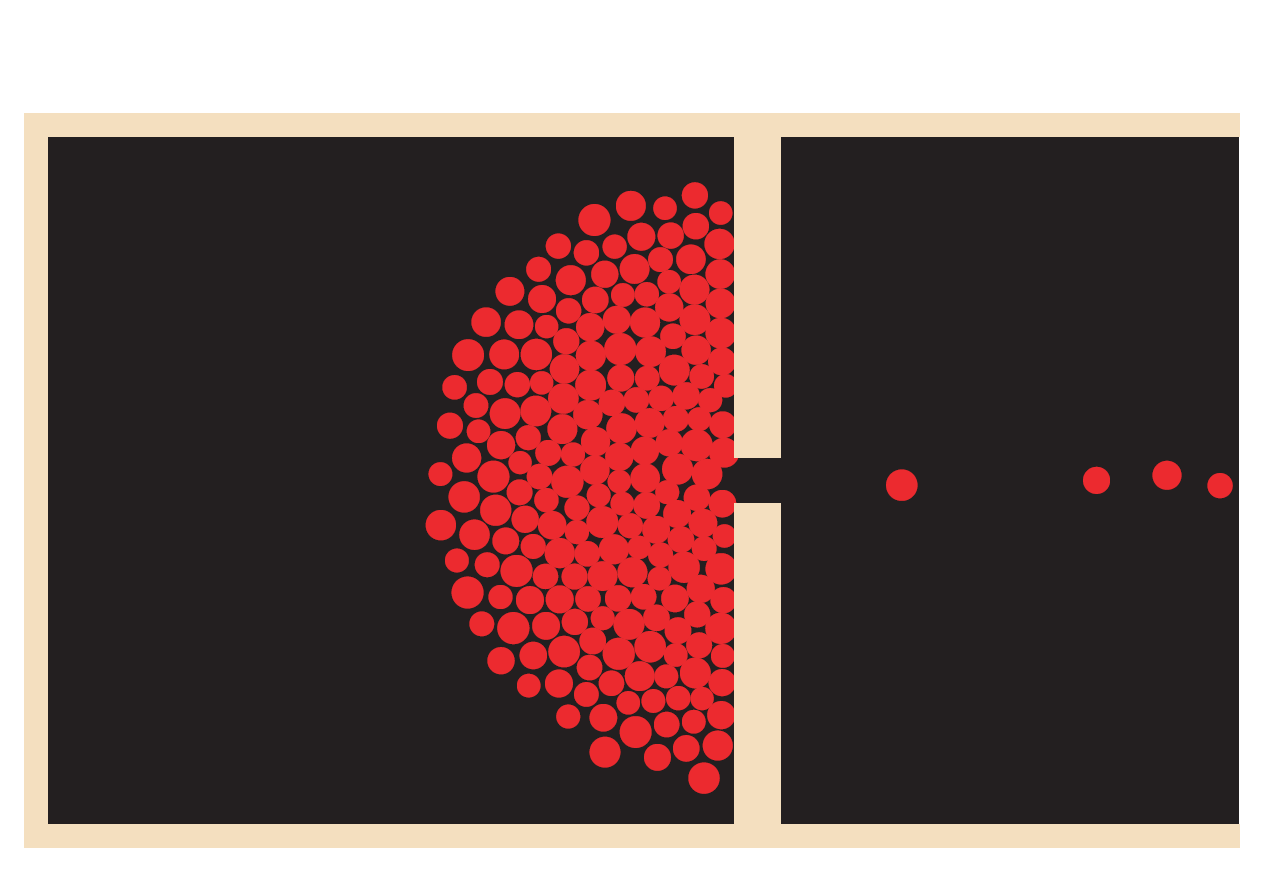
\includegraphics[width=0.45\textwidth]{Figures/square_room_letters.png}
        \label{subfig:fast-slow-clogging}
    }
    \subfloat[Leaving time versus desired velocity.]{
        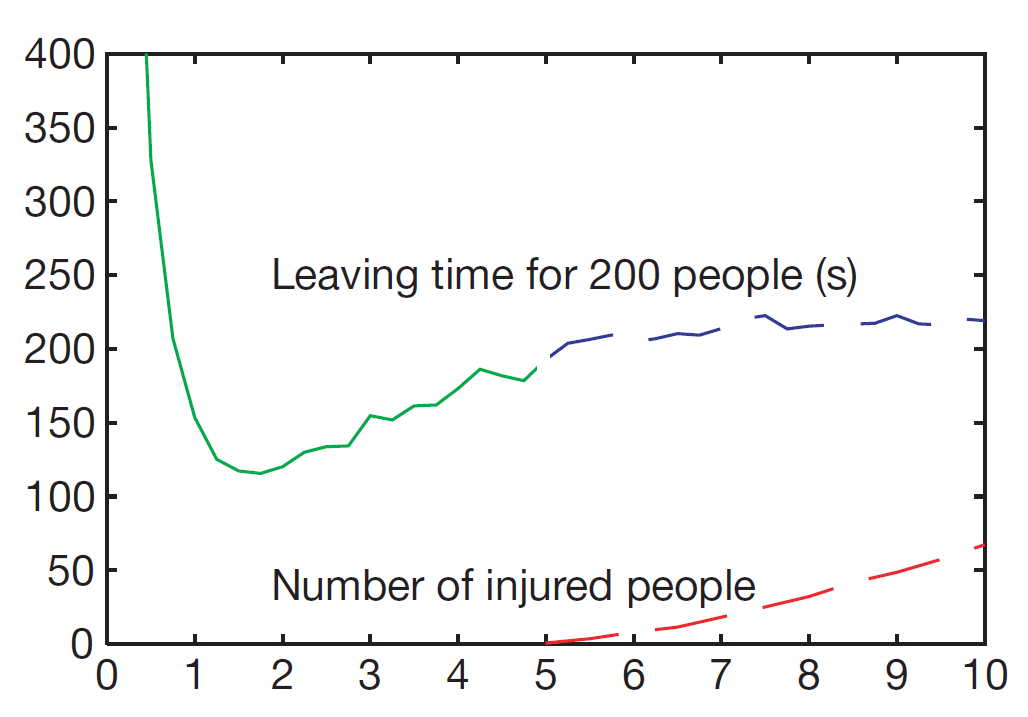
\includegraphics[width=0.45\textwidth]{Figures/leaving_time.png}
        \label{subfig:fast-slow-graph}
    }
    \caption[Faster-is-slower effect from \cite{helbing00}]{Faster-is-slower 
    effect from \cite{helbing00}. \subref{subfig:fast-slow-clogging} Clogging 
    occurs at doorways. \subref{subfig:fast-slow-graph} Fast desired 
    velocities leads to slower emptying of the room.}
    \label{fig:LtNFasterIsSlower}
\end{figure}

In our simulations of the square room scenario we have clogging in the 
doorways as expected (see figure~\ref{subfig:image-square-room}). We have 
plotted the time to leave the room as a function of the initial desired 
velocity with values from $0,5$ to $5,0$. As can be seen in 
figure~\ref{fig:square-room-leaving}, we do not see the leaving 
time increase with initial desired speed within any specific interval, although 
it is not a linear relationship between the velocity and 
leaving time either. Looking at the results, we conclude that we  do not see 
the faster-is-slower effect.

\begin{figure}[ht]
    \centering
    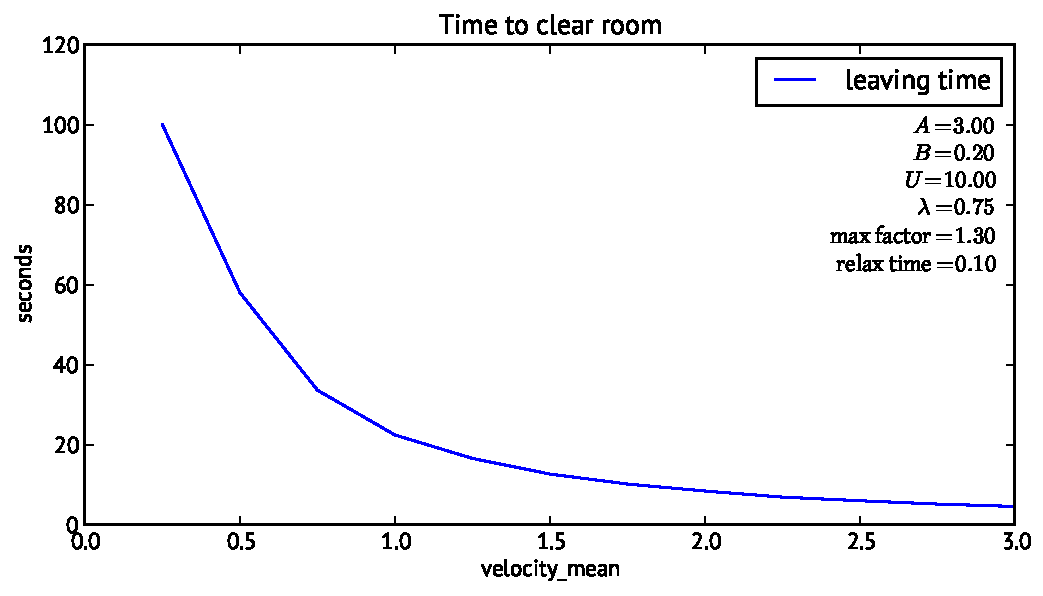
\includegraphics[width=0.8\textwidth]{Figures/timetoclearroom.pdf}
    \caption[Leaving time for the square room]{Leaving time for the square 
    room. We do not see the increase in leaving time as we increase the initial 
    desired speed.}
    \label{fig:square-room-leaving}
\end{figure}

\subsubsection{Freezing by heating effect}
The freezing by heating effect occurs when pedestrians are moving in opposite 
directions and they block each other when the initial desired velocity increases (see 
section~\ref{sec:article-results}). The illustration of this effect as 
presented in \cite{oscil} can be seen in 
figure~\ref{fig:freezing_by_heating_litterature}.

\begin{figure}[h]
    \centering
    \subfloat[]{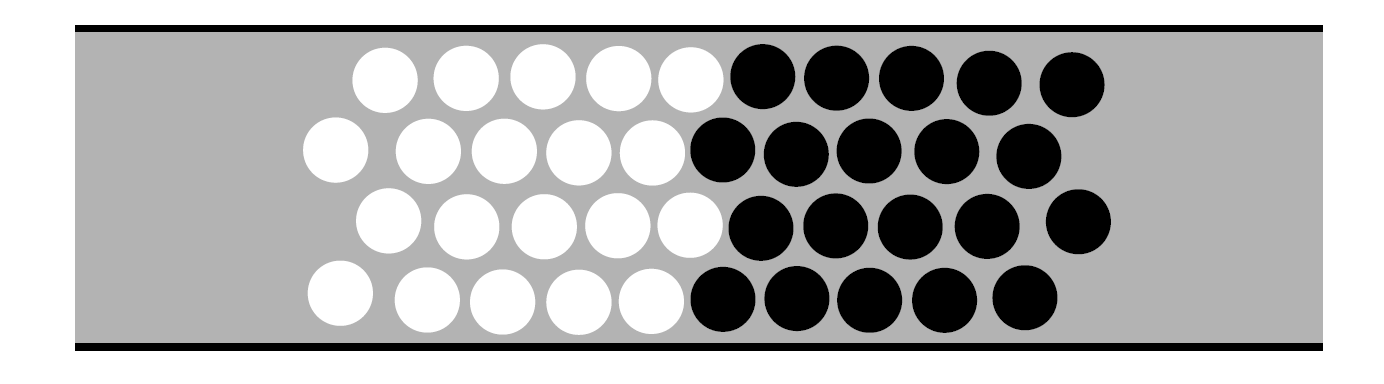
\includegraphics[width=0.45\textwidth]{Figures/heatfreeze.png}}
    \caption[Freezing by heating effect from \cite{oscil}]{Freezing by heating 
    effect from \cite{oscil}. Pedestrians block each other when the 
    freezing by heating phenomenon occurs.}
    \label{fig:freezing_by_heating_litterature}
\end{figure}

During our simulations we have not been able to reproduce this effect at all.  
Although we have seen clogging of corridors, it only occurs at low velocities, 
and so does not increase with the velocity as we expected. Instead, when 
pedestrians move faster, they are more likely to be able to pass each other 
even in corridors with high densities. So like the faster is slower
effect again we see no sign of a high desired velocity decreasing/stopping
the movement of the pedestrians.

\subsubsection{Lane formation}
Lane formation happens when the simulation contains bidirectional flow in 
corridors. As stated in \ref{self-org}:

\begin{quote}
    If pedestrians crowds moving in opposite directions meet each other, they 
    form small \emph{channels} in the beginning, but these channels later 
    merge to produce wide lanes
\end{quote}

An illustration of this phenomenon from \cite{lanes} can be seen in 
figure~\ref{fig:lanes-literature}. 

\begin{figure}[h]
    \centering
    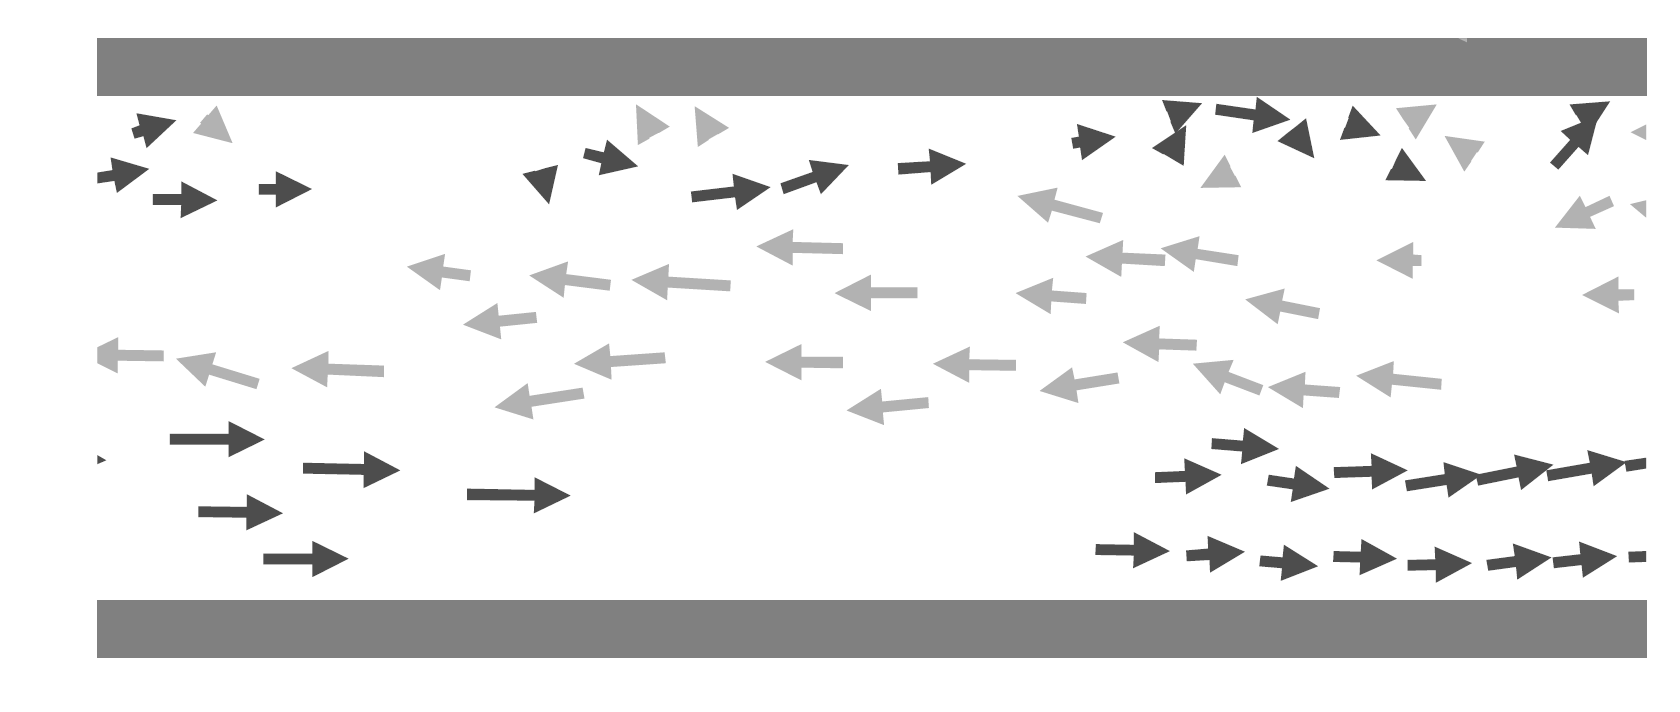
\includegraphics[width=0.8\textwidth]{Figures/flow_lanes_litterature.png}
    \caption[Lane formation from \cite{lanes}]{Lane formation from 
    \cite{lanes}. Pedestrians through a corridor form alternating lanes of 
    pedestrians going in each direction.}
    \label{fig:lanes-literature}
\end{figure}

Since we have three different corridor cases we have looked for lane
formation in all of them. As can be seen in figure~\ref{fig:laneformation}, 
the lane formation occurs in all of the cases.

\begin{figure}[h]
    \centering
    \subfloat[Bidirectional flow in a corridor.]{
        \resizebox{0.45\textwidth}{!}{\begin{tikzpicture}
\draw[color=blue] (-2.64,-1.02) circle (0.34);
\draw[color=blue] (-2.89,0.96) circle (0.31);
\draw[color=green] (5.10,-0.19) circle (0.32);
\draw[color=green] (2.19,0.17) circle (0.34);
\draw[color=green] (7.16,-1.49) circle (0.34);
\draw[color=green] (4.10,0.13) circle (0.28);
\draw[color=blue] (-5.87,0.58) circle (0.32);
\draw[color=green] (4.72,-1.57) circle (0.30);
\draw[color=blue] (-0.53,1.69) circle (0.30);
\draw[color=blue] (-2.13,1.68) circle (0.31);
\draw[color=blue] (-5.04,-0.15) circle (0.30);
\draw[color=green] (5.64,-1.69) circle (0.33);
\draw[color=green] (3.38,-1.57) circle (0.32);
\draw[color=blue] (-10.87,-1.75) circle (0.30);
\draw[color=green] (6.43,-0.42) circle (0.31);
\draw[color=green] (2.34,-1.60) circle (0.31);
\draw[color=blue] (-4.76,1.74) circle (0.33);
\draw[color=blue] (-8.66,1.76) circle (0.30);
\draw[color=blue] (-9.81,1.46) circle (0.31);
\draw[color=blue] (-3.52,1.75) circle (0.28);
\draw[color=blue] (-1.27,1.16) circle (0.25);
\draw[color=blue] (-2.06,0.63) circle (0.31);
\draw[color=green] (7.84,-1.70) circle (0.32);
\draw[color=blue] (-1.27,-0.56) circle (0.29);
\draw[color=blue] (-0.27,-0.60) circle (0.35);
\draw[color=green] (1.33,-1.66) circle (0.27);
\draw[color=green] (0.99,0.39) circle (0.30);
\draw[color=blue] (1.08,-0.61) circle (0.30);
\draw[color=blue] (-4.23,-0.62) circle (0.33);
\draw[color=blue] (-6.83,1.76) circle (0.33);
\draw[color=blue] (2.23,1.76) circle (0.29);
\draw[color=blue] (0.34,1.27) circle (0.28);
\draw[color=blue] (1.12,1.73) circle (0.30);
\draw[color=green] (-1.39,-0.16) circle (0.27);
\draw[color=green] (0.26,-1.60) circle (0.28);
\draw[color=green] (-3.13,0.14) circle (0.31);
\draw[color=blue] (5.12,-0.87) circle (0.32);
\draw[color=blue] (2.68,-0.64) circle (0.31);
\draw[color=blue] (4.72,1.61) circle (0.28);
\draw[color=green] (-0.92,-1.72) circle (0.29);
\draw[color=blue] (1.78,0.88) circle (0.28);
\draw[color=blue] (3.41,1.80) circle (0.31);
\draw[color=blue] (3.57,1.05) circle (0.33);
\draw[color=green] (-3.73,0.67) circle (0.32);
\draw[color=green] (-3.21,-1.68) circle (0.28);
\draw[color=green] (-4.56,-1.74) circle (0.29);
\draw[color=green] (-2.18,-1.73) circle (0.30);
\draw[color=green] (-6.02,-0.90) circle (0.31);
\draw[color=green] (-5.41,-0.54) circle (0.30);
\draw[color=blue] (8.22,-1.63) circle (0.30);
\draw[color=blue] (6.29,1.33) circle (0.34);
\draw[color=blue] (5.78,0.55) circle (0.27);
\draw[color=green] (-6.35,0.65) circle (0.28);
\draw[color=green] (-9.00,-1.11) circle (0.29);
\draw[color=blue] (6.83,-0.45) circle (0.34);
\draw[color=green] (-7.61,0.21) circle (0.34);
\draw[color=blue] (7.83,0.76) circle (0.28);
\draw[color=green] (-7.85,-1.11) circle (0.29);
\draw[color=green] (-9.23,0.34) circle (0.32);
\draw[color=green] (-8.66,-0.31) circle (0.31);
%\node at (-12.50, 5.83) {t = 10.12};
\useasboundingbox (-12.50, -5.83) rectangle (12.50, 5.83);
\draw[color=black] (-10.00,2.50) -- (10.00,2.50);
\draw[color=black] (-10.00,-2.50) -- (10.00,-2.50);
\end{tikzpicture}
}
    }
    \subfloat[Bidirectional flow in a corridor with a bottleneck.]{
        \resizebox{0.45\textwidth}{!}{\begin{tikzpicture}
\draw[color=blue] (-5.03,-1.14) circle (0.32);
\draw[color=blue] (-8.18,-1.13) circle (0.29);
\draw[color=blue] (-12.00,-0.90) circle (0.29);
\draw[color=blue] (-11.43,-1.43) circle (0.28);
\draw[color=blue] (-7.50,-0.61) circle (0.29);
\draw[color=blue] (-10.95,-0.73) circle (0.30);
\draw[color=blue] (-6.99,-1.13) circle (0.29);
\draw[color=blue] (-8.55,0.46) circle (0.29);
\draw[color=blue] (-3.37,-0.90) circle (0.29);
\draw[color=blue] (-6.46,0.83) circle (0.30);
\draw[color=green] (9.68,-0.09) circle (0.28);
\draw[color=green] (7.24,0.24) circle (0.29);
\draw[color=green] (8.09,-0.29) circle (0.31);
\draw[color=blue] (-1.95,0.74) circle (0.31);
\draw[color=blue] (-2.91,-0.60) circle (0.30);
\draw[color=blue] (-4.56,0.81) circle (0.29);
\draw[color=green] (6.58,-0.35) circle (0.30);
\draw[color=blue] (-6.57,-0.54) circle (0.29);
\draw[color=blue] (0.40,0.19) circle (0.30);
\draw[color=blue] (-8.24,1.03) circle (0.31);
\draw[color=green] (4.36,0.09) circle (0.31);
\draw[color=green] (5.12,-0.62) circle (0.29);
\draw[color=green] (6.32,0.45) circle (0.30);
\draw[color=green] (4.08,0.79) circle (0.30);
\draw[color=green] (3.85,-0.67) circle (0.30);
\draw[color=green] (5.71,-0.05) circle (0.30);
\draw[color=blue] (-1.45,0.19) circle (0.30);
\draw[color=blue] (1.44,-0.95) circle (0.32);
\draw[color=blue] (-2.38,-0.55) circle (0.29);
\draw[color=green] (3.56,0.11) circle (0.29);
\draw[color=green] (-1.76,0.10) circle (0.30);
\draw[color=blue] (-1.85,-0.67) circle (0.32);
\draw[color=green] (0.28,0.64) circle (0.32);
\draw[color=blue] (-1.22,-0.43) circle (0.29);
\draw[color=green] (-0.38,0.74) circle (0.30);
\draw[color=green] (-2.27,0.27) circle (0.31);
\draw[color=green] (-1.10,1.07) circle (0.31);
\draw[color=blue] (4.11,-1.40) circle (0.30);
\draw[color=green] (-1.88,1.32) circle (0.30);
\draw[color=green] (-3.72,-1.86) circle (0.29);
\draw[color=green] (-2.67,0.05) circle (0.30);
\draw[color=blue] (3.92,1.40) circle (0.31);
\draw[color=green] (-4.24,1.75) circle (0.29);
\draw[color=blue] (5.16,-1.32) circle (0.29);
\draw[color=green] (-5.12,0.08) circle (0.29);
\draw[color=green] (-6.04,1.97) circle (0.31);
\draw[color=blue] (7.08,1.47) circle (0.30);
\draw[color=green] (-6.81,2.11) circle (0.29);
\draw[color=blue] (7.23,0.72) circle (0.30);
\draw[color=blue] (7.43,-1.11) circle (0.32);
\draw[color=blue] (7.91,2.22) circle (0.29);
\draw[color=green] (-8.85,0.66) circle (0.29);
\draw[color=green] (-8.91,-2.45) circle (0.30);
\draw[color=green] (-9.52,-1.90) circle (0.29);
%\node at (-12.50, 5.83) {t = 18.99};
\useasboundingbox (-12.50, -5.83) rectangle (12.50, 5.83);
\draw[color=black] (-10.00,3.00) -- (-5.00,3.00);
\draw[color=black] (-10.00,-3.00) -- (-5.00,-3.00);
\draw[color=black] (-5.00,3.00) -- (0.00,1.00);
\draw[color=black] (-5.00,-3.00) -- (0.00,-1.00);
\draw[color=black] (0.00,1.00) -- (5.00,3.00);
\draw[color=black] (0.00,-1.00) -- (5.00,-3.00);
\draw[color=black] (5.00,3.00) -- (10.00,3.00);
\draw[color=black] (5.00,-3.00) -- (10.00,-3.00);
\end{tikzpicture}
}
    }\\
    \subfloat[Bidirectional flow in a corridor with a widening.]{
        \resizebox{0.45\textwidth}{!}{\begin{tikzpicture}
\draw[color=green] (12.32,-0.03) circle (0.31);
\draw[color=blue] (-10.02,-0.69) circle (0.30);
\draw[color=green] (11.41,0.08) circle (0.27);
\draw[color=blue] (-10.66,0.64) circle (0.31);
\draw[color=blue] (-7.02,-0.60) circle (0.32);
\draw[color=blue] (-6.37,-0.56) circle (0.30);
\draw[color=blue] (-12.06,0.27) circle (0.32);
\draw[color=blue] (-9.95,0.69) circle (0.30);
\draw[color=green] (1.97,-0.54) circle (0.29);
\draw[color=green] (8.89,0.24) circle (0.30);
\draw[color=blue] (-9.06,0.69) circle (0.31);
\draw[color=blue] (-6.57,0.59) circle (0.30);
\draw[color=blue] (-3.43,1.33) circle (0.29);
\draw[color=blue] (-9.41,-0.70) circle (0.28);
\draw[color=blue] (-5.34,-0.64) circle (0.29);
\draw[color=green] (7.67,0.09) circle (0.29);
\draw[color=blue] (-4.51,-0.92) circle (0.28);
\draw[color=green] (5.68,-0.36) circle (0.29);
\draw[color=blue] (-2.27,1.75) circle (0.29);
\draw[color=blue] (-4.37,0.95) circle (0.30);
\draw[color=blue] (-3.71,-1.20) circle (0.30);
\draw[color=blue] (-2.44,1.02) circle (0.29);
\draw[color=blue] (-1.46,0.87) circle (0.29);
\draw[color=blue] (0.65,-1.58) circle (0.29);
\draw[color=blue] (-0.52,1.03) circle (0.30);
\draw[color=green] (3.00,0.01) circle (0.28);
\draw[color=green] (1.45,-0.27) circle (0.29);
\draw[color=green] (0.56,-0.27) circle (0.31);
\draw[color=blue] (0.70,1.06) circle (0.31);
\draw[color=blue] (1.35,-1.29) circle (0.30);
\draw[color=blue] (1.66,1.29) circle (0.29);
\draw[color=green] (-0.51,-0.20) circle (0.30);
\draw[color=blue] (1.99,-0.92) circle (0.29);
\draw[color=blue] (3.79,0.43) circle (0.30);
\draw[color=blue] (1.03,0.46) circle (0.31);
\draw[color=green] (-1.49,-0.03) circle (0.31);
\draw[color=green] (-2.00,-0.58) circle (0.29);
\draw[color=green] (-2.13,0.43) circle (0.30);
\draw[color=green] (-2.97,0.31) circle (0.30);
\draw[color=green] (-3.49,-0.26) circle (0.30);
\draw[color=green] (-4.02,0.25) circle (0.30);
\draw[color=blue] (4.55,0.37) circle (0.30);
\draw[color=blue] (6.26,-0.63) circle (0.32);
\draw[color=blue] (5.51,0.45) circle (0.29);
\draw[color=green] (-4.97,0.10) circle (0.29);
\draw[color=green] (-7.00,-0.21) circle (0.30);
\draw[color=blue] (6.76,-0.50) circle (0.32);
\draw[color=green] (-7.32,0.18) circle (0.32);
\draw[color=blue] (7.56,-0.38) circle (0.29);
\draw[color=green] (-8.15,0.08) circle (0.30);
\draw[color=green] (-8.88,-0.25) circle (0.31);
\draw[color=green] (-9.16,0.29) circle (0.31);
\draw[color=blue] (9.51,-0.32) circle (0.30);
\node at (-12.50, 5.83) {t = 19.99};
\useasboundingbox (-12.50, -5.83) rectangle (12.50, 5.83);
\draw[color=black] (-10.00,1.00) -- (-5.00,1.00);
\draw[color=black] (-10.00,-1.00) -- (-5.00,-1.00);
\draw[color=black] (-5.00,1.00) -- (0.00,3.00);
\draw[color=black] (-5.00,-1.00) -- (0.00,-3.00);
\draw[color=black] (0.00,3.00) -- (5.00,1.00);
\draw[color=black] (0.00,-3.00) -- (5.00,-1.00);
\draw[color=black] (5.00,1.00) -- (10.00,1.00);
\draw[color=black] (5.00,-1.00) -- (10.00,-1.00);
\end{tikzpicture}
}
    }
    \caption[Lane formation in corridor simulations]{Lane formation in 
    corridor simulations. The colours indicate the direction the pedestrians 
    are moving in. The blue ones are walking to the left; the green ones 
    are walking to the right. Lane formation can be seen in all three cases. }
    \label{fig:laneformation}
\end{figure}

\subsubsection{Oscillating flows}
Oscillating flows occur when clogging occurs at a bottleneck, and small groups 
of pedestrians from each direction alternate in getting through the 
bottleneck. The effect is described in \cite{oscil}, but it is not clear how 
they measure it. Figure~\ref{fig:oscillitoryflow_litterature} shows the 
illustration from the article that explains the effect.

When looking at the simulation while it is running it is not immediately clear 
whether the oscillatory flow occurs. Clogging appears in both ends of the 
bottleneck and people are sometimes squeezed through the bottleneck. To get a 
better indication of whether or not oscillation occurs, we have graphed the 
flow rate in each direction. This graph is seen in 
figure~\ref{fig:oscillatory-flow}. The graph does not show a clear indication 
of oscillating flows, however a possible source of error is that the flow rate 
is measure at the ends of the corridor, which may dilute the effect as 
pedestrians are passing through the crowd after having passed through the 
bottleneck. However, in the way our simulation is implemented, it is not 
possible to distinguish between pedestrians moving in different directions 
when measuring the flow rate in the middle of the bottleneck.

In conclusion, we may be able to replicate the oscillating flows, but the 
results are not completely clear.
\begin{figure}[h]
    \centering
    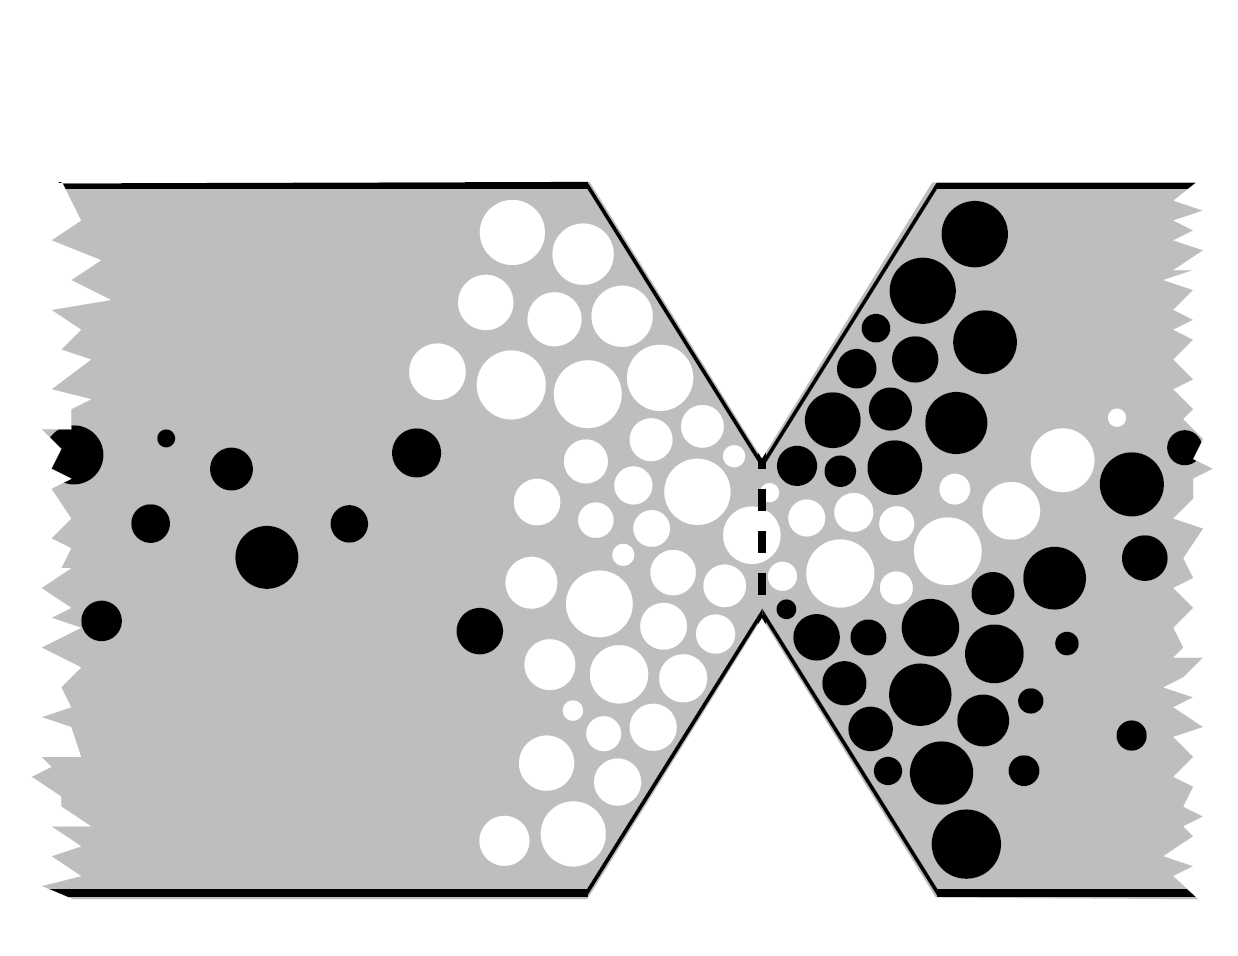
\includegraphics[width=0.4\textwidth]{Figures/oscil_flow.png}
    \caption[Illustration of oscillating flow from \cite{oscil}]{Illustration 
    of oscillating flow from \cite{oscil}. A small group of pedestrians 
    slipping through the bottleneck passes through the bottleneck in one 
    direction. Oscillations occur when pedestrians alternately pass through 
    the bottleneck from each direction.}
    \label{fig:oscillitoryflow_litterature}
\end{figure}

\begin{figure}[h]
    \centering
    \subfloat[Flowrates measured at each end of the corridor]{
        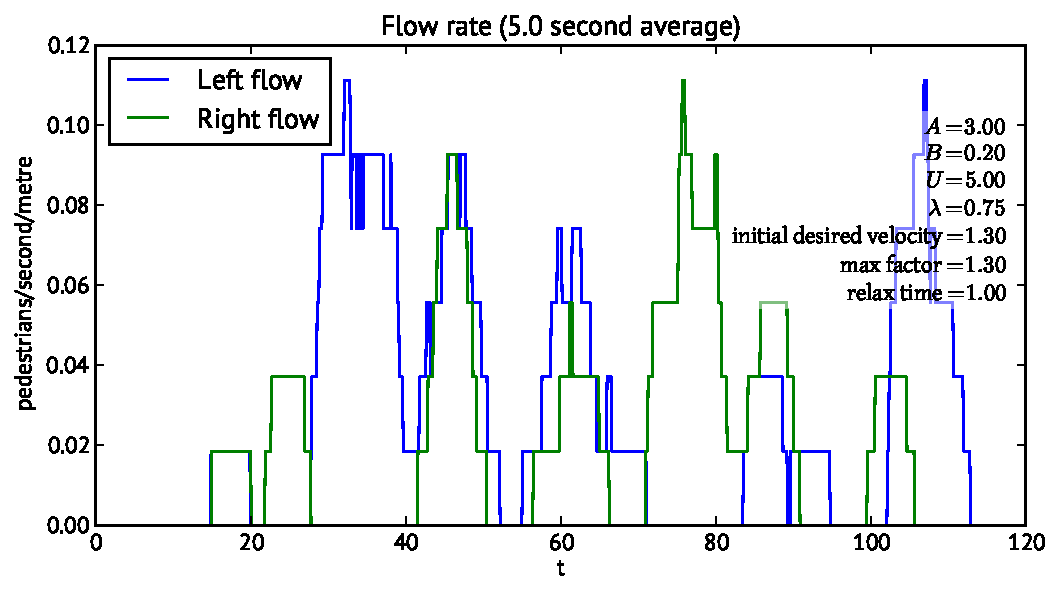
\includegraphics[width=0.45\textwidth]{Figures/flowrateBiDirecBottle.pdf}
        \label{subfig:flow-graph}
    }
    \subfloat[Clogging of a bottleneck]{
        \resizebox{0.45\textwidth}{!}{\begin{tikzpicture}
\draw[color=green] (-1.76,-0.12) circle (0.30);
\draw[color=blue] (0.64,-0.77) circle (0.30);
\draw[color=blue] (0.10,0.27) circle (0.30);
\draw[color=green] (-0.37,-0.03) circle (0.30);
\draw[color=blue] (1.17,0.92) circle (0.30);
\draw[color=blue] (1.87,-0.30) circle (0.30);
\draw[color=blue] (0.55,0.67) circle (0.30);
\draw[color=blue] (1.64,0.42) circle (0.30);
\draw[color=blue] (-4.68,-1.58) circle (0.30);
\draw[color=green] (1.32,-0.23) circle (0.30);
\draw[color=green] (0.85,0.04) circle (0.30);
\draw[color=green] (-0.52,-0.70) circle (0.30);
\draw[color=green] (-0.40,0.73) circle (0.30);
\draw[color=green] (-1.35,-0.68) circle (0.30);
\draw[color=green] (0.30,-0.35) circle (0.30);
\draw[color=blue] (1.97,1.10) circle (0.30);
\draw[color=blue] (1.34,-0.95) circle (0.30);
\draw[color=blue] (2.46,0.40) circle (0.30);
\draw[color=green] (-0.97,0.21) circle (0.30);
\draw[color=green] (-2.66,0.11) circle (0.30);
\draw[color=blue] (2.50,-0.53) circle (0.30);
\draw[color=green] (-1.35,0.87) circle (0.30);
\draw[color=blue] (1.97,-1.16) circle (0.30);
\draw[color=green] (-1.99,0.89) circle (0.30);
\draw[color=green] (-4.08,-0.52) circle (0.30);
\draw[color=green] (-3.93,0.62) circle (0.30);
\draw[color=blue] (7.18,-1.19) circle (0.30);
\draw[color=green] (-7.18,1.24) circle (0.30);
\draw[color=green] (-8.93,-1.69) circle (0.30);
\draw[color=green] (-9.49,-0.01) circle (0.30);
\node at (-12.50, 5.83) {t = 63.00};
\useasboundingbox (-12.50, -5.83) rectangle (12.50, 5.83);
\draw[color=black] (-10.00,3.00) -- (-5.00,3.00);
\draw[color=black] (-10.00,-3.00) -- (-5.00,-3.00);
\draw[color=black] (-5.00,3.00) -- (0.00,1.00);
\draw[color=black] (-5.00,-3.00) -- (0.00,-1.00);
\draw[color=black] (0.00,1.00) -- (5.00,3.00);
\draw[color=black] (0.00,-1.00) -- (5.00,-3.00);
\draw[color=black] (5.00,3.00) -- (10.00,3.00);
\draw[color=black] (5.00,-3.00) -- (10.00,-3.00);
\end{tikzpicture}
}
        \label{subfig:bottleneck}
    }\\
    
    \caption[Oscillatory flow simulations]{Oscillatory flow simulations. 
    \subref{subfig:flow-graph} Flowrates measured at each end of the corridor 
    of a simulation. While there is some alternating behaviour it is not clear 
    whether oscillatory flow occurs. \subref{subfig:bottleneck} Clogging at a 
    bottleneck when pedestrians approach it from both directions.}
    \label{fig:oscillatory-flow}
\end{figure}

\subsection{Summary}
We have seen that our simulation is able to show reasonable results of 
pedestrians moving through our chosen scenarios. We have simulated four 
different scenarios, and tried to replicate the results presented in the 
literature. We have not been able to replicate either the faster-is-slower 
effect or freezing by heating. Lane formation we do see, and it is unclear 
whether oscillatory flows are seen, perhaps partly because our way of 
measuring this is not very good.
